\documentclass[a4paper,10pt]{article}
\usepackage{fontspec}
\usepackage{setspace}
\usepackage{booktabs}
\usepackage{amsmath}
\usepackage{cancel}
\usepackage{graphicx}
\usepackage{biblatex}
\usepackage{float}

\setmainfont{arial}
\setstretch{1.15}
\addbibresource{references.bib}

\title{Depth estimation using neural network}
\author{Arif Suganda\\
        Tadulako University\\
        \texttt{f5522530002@untad.ac.id}
}

\begin{document}
\maketitle

\section{Introduction}
Depth estimation (DE) is a fundamental problem in operating an artificial intelligence system, such as robotics, autonomous vehiche, and augmented reality in real world.
Computer understanding of spatial context is called ``depth information'', and it have been solved by relying on hardware-heavy solution such as LiDAR (Light Detection and Ranging) and Time-of-Flight (ToF) sensors.
While these hardware solutions are accurate, it is expensive, bulky and consume a huge number of power. 
Just as humans see the spatial information using our eyes and brain, the purpose of this reseach is to explore the capability of computers to estimate depth information only using an image cues.

The implementation of depth estimation can be functionally classified into three divisions, including monocular depth estimation (MDE), binocular depth estimation (BDE), or multi-view depth estimation (MVDE)~\cite{Masoumian2022MDEReview}.
The earlier research of depth estimation focused heavily on stereo vision, inspired by human binocular perception.
Stereo vision works by estimating the depth from disparities between two calibrated cameras~\cite{Zhang2025MDESurvey}.
While Multi-view methods acquire depth information by utilising visual cues and different camera parameters~\cite{Khan2020MDEReview}.

Implementation of stereo and multi-view required a high computational time, memory and cost due to the usage of multiple sensors and processes.
These requirements have limit their practicality and implementation in application~\cite{Khan2020MDEReview,Masoumian2022MDEReview}, this leaves us with monocular depth estimation (MDE) approach.

Monocular depth estimation from Red-Green-Blue (RGB) images is a well-stud-ied ill-posed problem in computer vision which has been investigated intensively over the past decade using Deep Learning (DL) approaches~\cite{Khan2020MDEReview}.
Ill-posed problem in MDE means that there are no concrete solution to solve a depth estimation using only single image, because there are no references to determined the solution of MDE problem.
MDE research is heavily dominated by deep learning (DL) model~\cite{Masoumian2022MDEReview}. Since eigen~\cite{eigen14062283}, convolutional neural networks (CNNs) have been the primary architecture used in depth estimation, there are also variety architecture such as encoder-decoder model, residual networks, generative adversarial model and transformer-based model.

\subsection{Research purpose}
The purpose of this research is to explore the capability of a computer system to estimate the depth information using only an image cues.
This research will be focused on monocular depth estimation (MDE) using deep learning (DL) model.

\section{Methodology}

\subsection{Dataset}
The dataset used in this research is the KITTI dataset~\cite{Geiger2013IJRR}, which is a widely used benchmark for depth estimation tasks.

\subsection{Network architecture}

\subsection{Evaluation}

\section{Experiment}
The experiment is conducted following the configuration as follows.
\begin{enumerate}
        \item The dataset images and depth maps have a resolution of 192x640 pixels.
        \item The model is trained for 10 epochs with a batch size of 16.
        \item The training is performed on a Macbook Pro with M1 Pro chip.
\end{enumerate}

\subsection{Implementation}
Experiment is conducted to explore the deep learning model for monocular depth estimation.
The results of the experiment is shown in Figure~\ref{fig:comparison}, where the left image is the original RGB image and the right image is the predicted depth map generated by the model.

\begin{figure}[H]
    \centering
    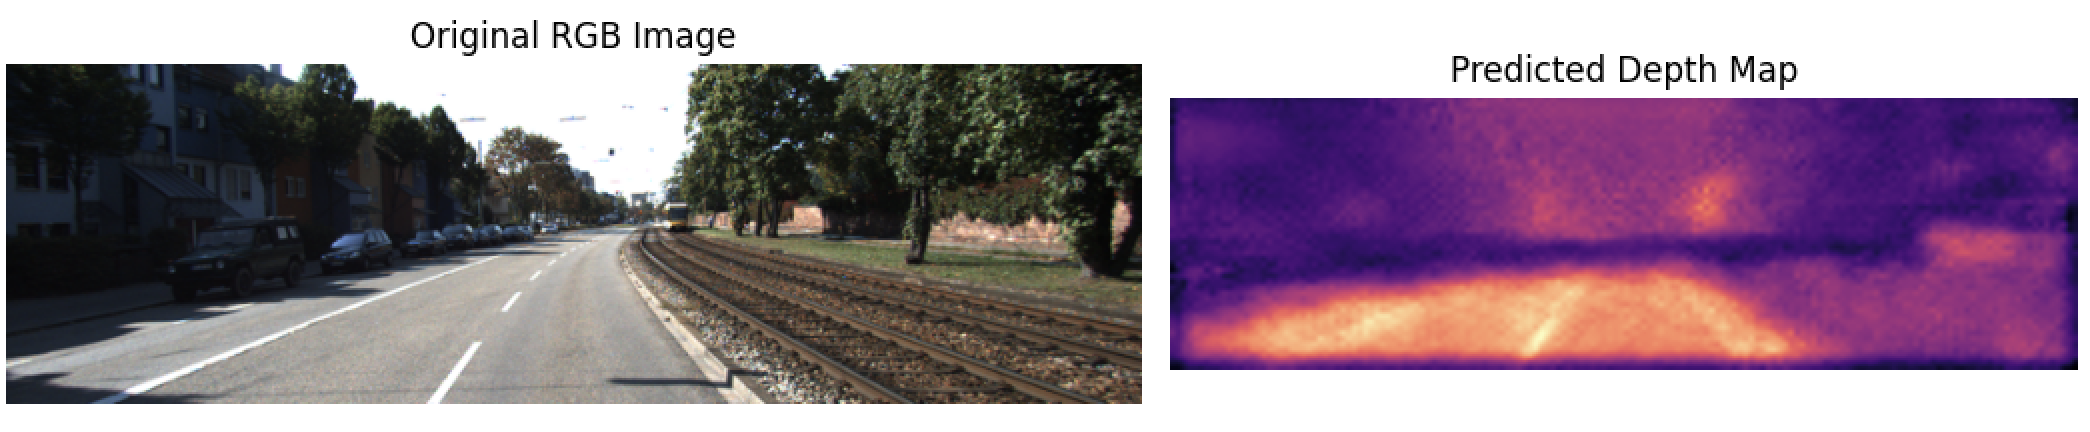
\includegraphics[width=1\textwidth]{comparison.png} 
    \caption{Comparison of Original RGB Image and Predicted Depth Map}\label{fig:comparison}
\end{figure}

\subsection{Metrics}

\section{Discussion}

\end{document}